\chapter{Métodos Iterativos}
Como ya hemos visto, los métodos directos poseen en general una complejidad de orden cúbico en el número de incógnitas $\mathcal{O}(N^3)$. Esto dice que si en un problema determinado se duplica el número de incógnitas entonces el número de operaciones se multiplica por 8. Eso ha llevado a intentar desarrollar métodos de orden menor \footnote{Observe que el límite inferior para un método de resolución  es $\mathcal{O}(N^2)$ ya que ese es el número de coeficientes de la matriz.} y los métodos iterativos son una posible alternativa.

Hay, además de la complejidad,  otros problemas con los métodos directos. Por ejemplo, en muchas aplicaciones aparecen problemas con un número muy grande de incógnitas pero con matrices \emph{ralas}, es decir, matrices con un elevado porcentaje de coeficiente nulos. Esto permite en principio reducir notablemente el número de operaciones del algoritmo pero sin embargo como desventaja aparece un ``rellenado'' innecesario en la factorización resultante. Veamos un ejemplo sencillo.

\section{Ejemplo: temperatura en una pieza de motor}
Ciertas ecuaciones lineales en derivadas parciales pueden resolverse de modo aproximado a través de discretizaciones. En la Figura \ref{fig:disc_piston} se muestra un cuarto de pistón (pieza que se desplaza dentro de uno de los cilindros de un motor).La distribución de temperatura en esa pieza puede calcularse resolviendo la ecuación del calor.
\begin{figure}[h]
\centering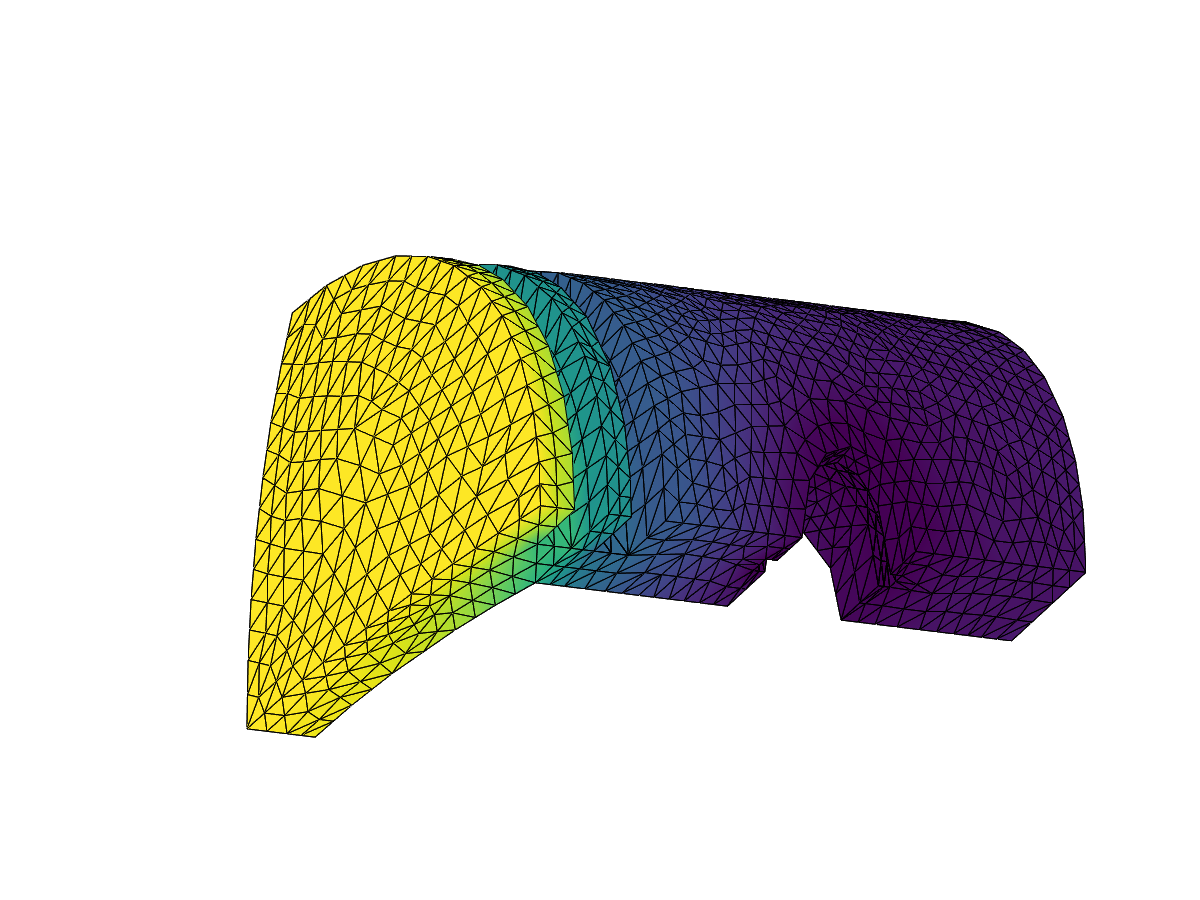
\includegraphics[width=0.4\linewidth]{piston.png}
\label{fig:disc_piston}
\end{figure}
Una vez discretizado, el problema puede escribirse como un sistema lineal. En este ejemplo particular, el sistema resultante  puede escribirse de la forma
 $$
 \Ab\xb=\bb,
 $$
 donde
 $$\Ab\in \R^{3319\times 3319}$$
cada incógnita es el valor de la temperatura en un nodo. En este problema la matriz resulta rala. En la Figura
\begin{figure}[h]
\centering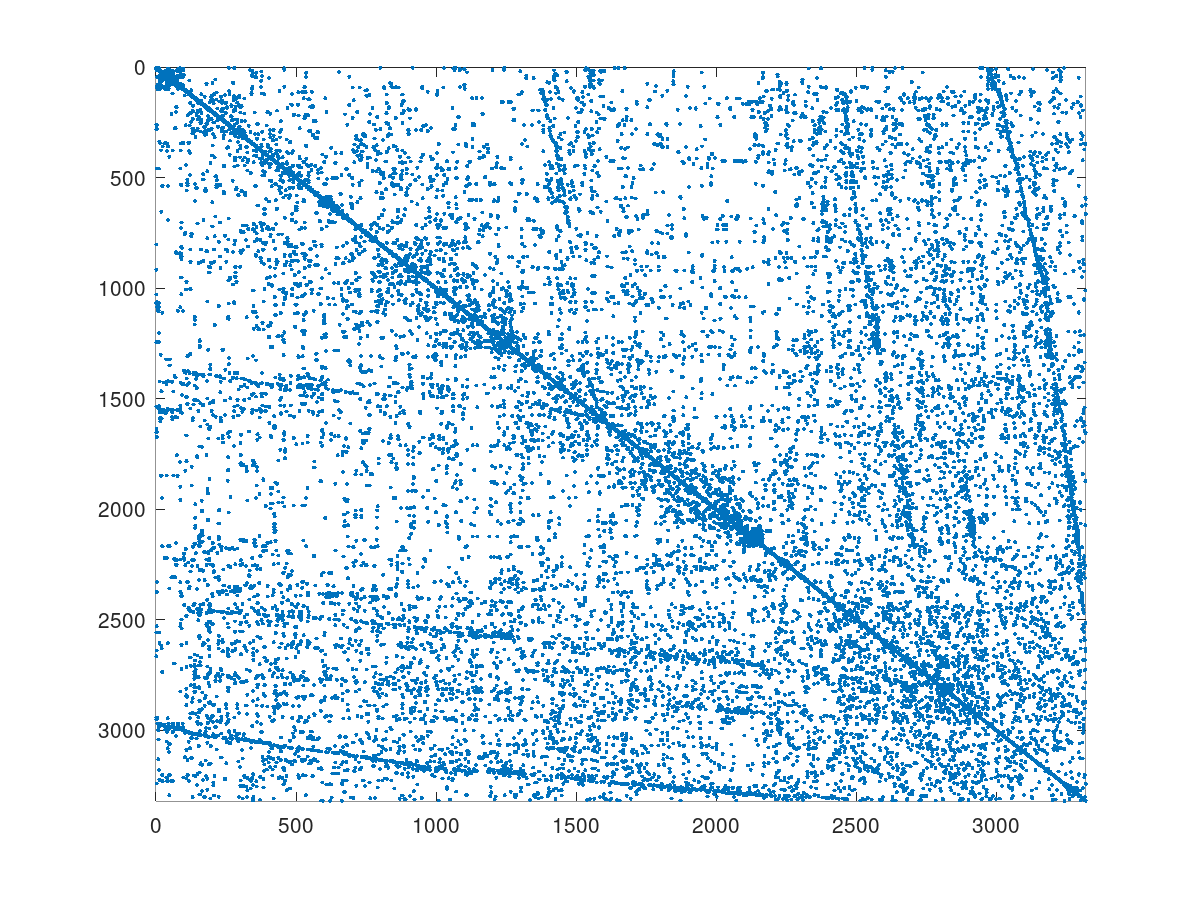
\includegraphics[width=0.6\linewidth]{matrizA.png}
\label{fig:matrizA}
\end{figure}
vemos (con el comando np.spy) que un numero grande de elementos de la matriz es nulo. De hecho, en este caso solamente $39753$ coeficientes son diferentes de cero, en vez $3319^2=11015761$. Desde  el punto de vista de la memoria utilizada en el almacenamiento de $\Ab$ esto es significativo. Teniendo en cuenta que en doble precisión cada número ocupa 8 bytes tendriamos en cada caso:
\begin{itemize}
 \item $39753\frac{8}{1024}\sim 300K$
 \item $11015761 \frac{8}{(1024)^2}\sim 84M$.
\end{itemize}
Esta ventaja se puede perder al hacer $LU$.
En efecto, en este ejemplo, a pesar de que $A$ tiene solo $39753$ elementos no nulos, el número de elementos no nulos de $L$ es $2440542$ ($\sim 18M$). Este fenómeno se conoce como rellenado. La apariencia de $L$ puede verse en la Figura

\begin{figure}[h]
\centering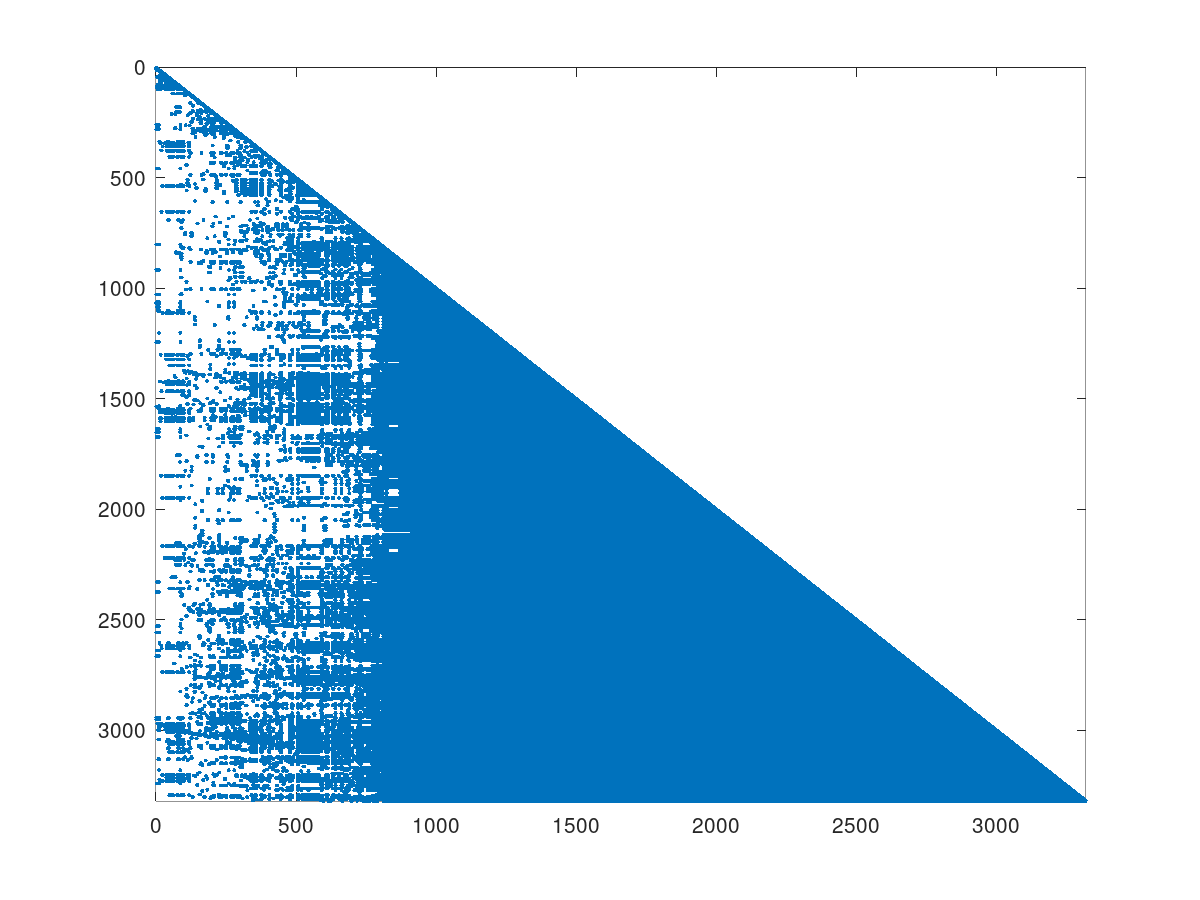
\includegraphics[width=0.6\linewidth]{matrizL.png}
\end{figure}



\begin{figure}[h]
\centering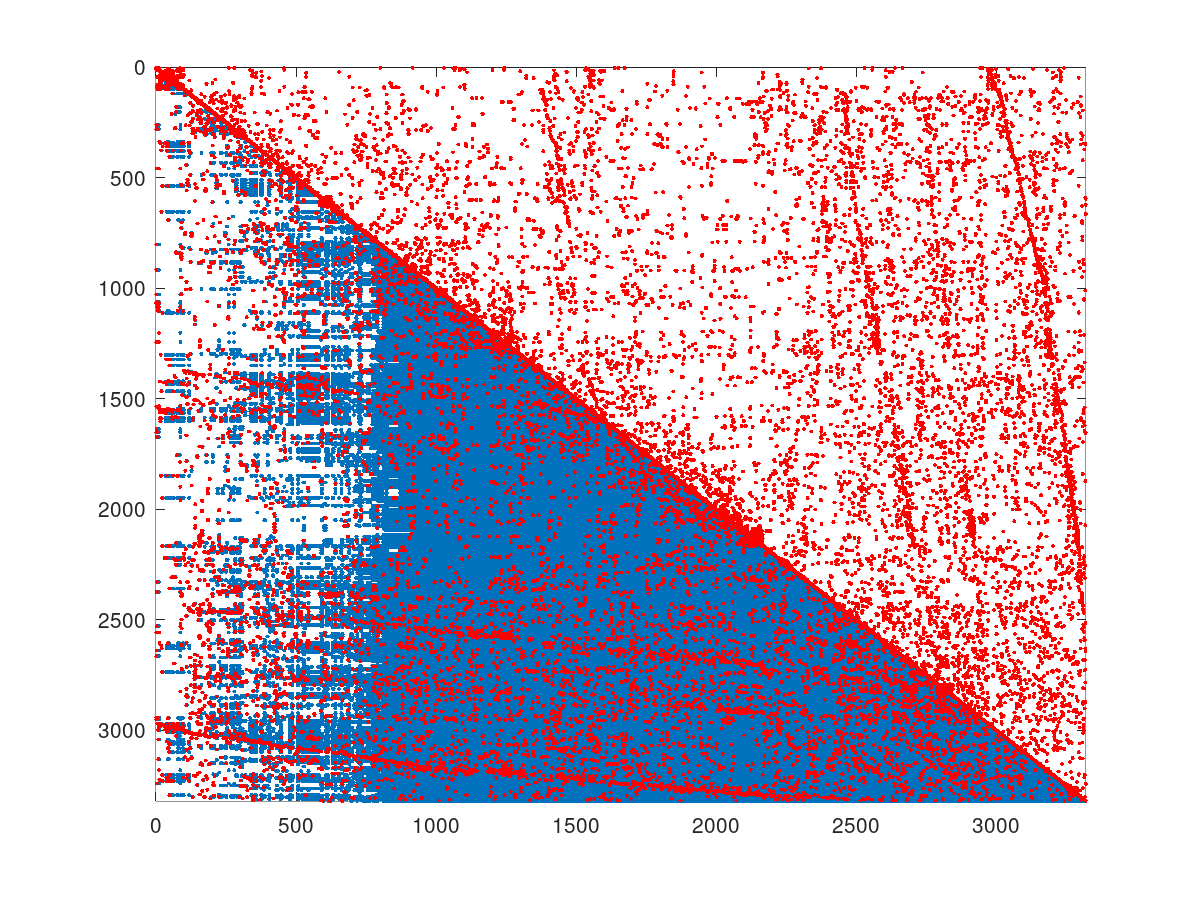
\includegraphics[width=0.6\linewidth]{matricesAyL.png}
\end{figure}


Si bien hay heurísticas para evitar el rellenado, buscando permutar las variables y las ecuaciones no las vamos a comentar por falta de tiempo. La alternativa que estudiaremos es la de los métodos iterativos. Estos no buscan ninguna factorización y se basan en iterar un procedimiento de orden $\mathcal{O}(N^2)$ (básicamente el producto de una matriz por vector mas una suma de dos vectores) unas pocas veces y conseguir una buena aproximación de la solución buscada.


Ya hemos visto que $\rho(\Ab)$ no es una norma, sin embargo verifica:
$$\rho(\Ab)\le \|\Ab\|,$$
para toda norma matricial $\|\cdot\|$.
Es decir:
$$
\rho(\Ab)\le\inf_{\|\cdot\|} \|\Ab\|.
$$

En realidad vale algo mas fuerte:
$$
\rho(\Ab)=\inf_{\|\cdot\|} \|\Ab\|.
$$
Lo que implica que para todo $0<\varepsilon$ existe una norma $\|\cdot\|$ tal que
$$\|\Ab\|\le \rho(\Ab)+ \varepsilon$$


Dada una matriz $\Mb\in \Knn$ nos interesa ver en que casos
$$
\lim_{k\to \infty}
\|\Mb^k\|=0
$$
notamos que:
\begin{itemize}
 \item Si existe $\|\cdot\|$ tal que
 $\|\Mb\|\le \mu <1$ entonces $\lim_{k\to \infty}
\|\Mb^k\|=0$, pues

$$\|\Mb^k\|\le \|\Mb\|^k\le \mu^k\to 0.$$
\end{itemize}


\tcc
\begin{prop}
 Sea $\Mb\in \Knn$, se tiene que
 $$
 \lim_{k\to \infty}\|\Mb^k\|=0
 $$
para cierta norma $\|\cdot\|$ sí y solo sí
 $\rho(\Mb)<1$.
\end{prop}

\etcc

\begin{proof}
 Si $\rho(\Mb)<1$, entonces existe $\|\cdot\|$ tal que $\|\Mb\|=\mu<1$ y listo.

 Por otro lado,
 $$
 \rho(\Mb)^k=
 \rho(\Mb^k)\le
 \|\Mb^k\|\ \to 0,
 $$
 de donde
 necesariamente
 $\rho(\Mb)<1$.
\end{proof}

\tcc
\begin{prop}
 Para toda norma subordinada $\|\cdot\|$ vale que
 $$
 \rho(\Mb)=\lim_{k\to \infty} \|\Mb^k\|^{1/k}.
 $$
\end{prop}

\etcc


\begin{proof}
 Dado $\epsilon>0$ existe una norma subordinada $\|\cdot\|_{*}$ tal que
 $$
 \|\Mb\|_{*}\le \rho(\Mb)+\epsilon.
 $$
 $$
 \rho(\Mb)^k=\rho(\Mb^k)\le \|\Mb^k\|\le C \|\Mb^k\|_{*}\le C \|\Mb\|^k_{*}\le C(\rho(\Mb)+\epsilon)^k,
 $$
 $$
 \rho(\Mb)\le \|\Mb^k\|^{1/k}\le C^{1/k}(\rho(\Mb)+\epsilon)
 $$
 tomando límite y notando que $\epsilon$ es arbitrario se demuestra el resultado.
\end{proof}

\begin{center}
 { \centering {Métodos Iterativos
}}
\end{center}

\begin{itemize}
 \item Se \emph{aproxima } la solución y no tiene en principio finitos pasos.
 \item A pesar de lo anterior uno espera tener aproximaciones comparables a las de los métodos directos con un costo  $<<\mathcal{O}(N^3)$.
\end{itemize}


Queremos resolver
$$
\Ab\xb=\bb,
$$
proponemos
$$\Ab=\Bb+\Cb,$$
donde $\Bb$ es \emph{fácil} de invertir y escribimos
$$
\Bb\xb=-\Cb\xb+\bb
$$
equivalentemente
$$
\xb=-\Bb^{-1}\Cb\xb+\Bb^{-1}\bb
$$


llamo

$\Mb_I=-\Bb^{-1}\Cb$ y $\Bb^{-1}\bb=\tilde{\bb}$

Resolver el sistema equivale a hallar $\xb$ tal que
$$
\xb=\Mb_I\xb+\tbb
$$
La idea de muchos métodos iterativos es tomar $\xb_0$ e iterar
$$
\xb_{n+1}=\Mb_I\xb_n+\tbb,
$$
bajo que condiciones $\xb_k\to \xb$?.

Estudiamos el error $\eb_k=\xb-\xb_k$
$$
\eb_{k+1}=\Mb_I\eb_k=\Mb_I\Mb_I\eb_{k-1}=\cdots = \Mb^{k+1}\eb_0
$$
es decir
$$\eb_k\to \cero$$
para todo $\eb_0$ sí y solo sí
$$\Mb_I^{k}\to \cero $$

pero
$$\Mb_I^{k}\to \cero $$
sí y solo sí
$$
\rho(\Mb_I)<1.
$$

Más aún
$$
\|\eb_k\|\le C\rho(\Mb_I)^k
$$
lo que nos dá la velocidad de convergencia del algoritmo.

$$\Bb=\omega^{-1}\Ib, \qquad \omega>0.$$
$$\Cb=\Ab-\omega^{-1}\Ib=\omega^{-1}(\omega\Ab-\Ib)$$
$$
\Mb_I=-\Bb^{-1}\Cb=
\Ib-\omega\Ab
$$
Método de Richardson.

\tcc
\begin{prop}
Si $\Ab$ es SDP, el método de Richardson converge -para todo dato inicial- sí y solo sí $\omega<\frac{2}{\rho(\Ab)}.$
\end{prop}
\etcc

\begin{proof}
 Basta ver bajo que condiciones $\rho(\Mb_I)<1$, con $
\Mb_I=
\Ib-\omega\Ab.
$ Como $\Ab$ es SDP sus autovalores cumplen $0<\lambda_1\le \lambda_2\le \cdots \le \lambda_n$. Los autovalores de $
\Mb_I$ son $1-\omega\lambda_i$, queremos
$
|1-\omega\lambda_i|<1,
$
$$
-1< 1-\omega\lambda_i< 1
$$
i.e. $\omega<\frac{2}{\lambda_i}$ para todo $1\le i\le n$ lo que equivale a
$\omega<\frac{2}{\rho(\Ab)}.$
\end{proof}

El óptimo $\omega$?. Sabemos que
$$
\rho(\Mb_I)=\max\{
|1-\omega   \lambda_n|,|1-\omega   \lambda_1|\}
$$
\begin{figure}[h]
\centering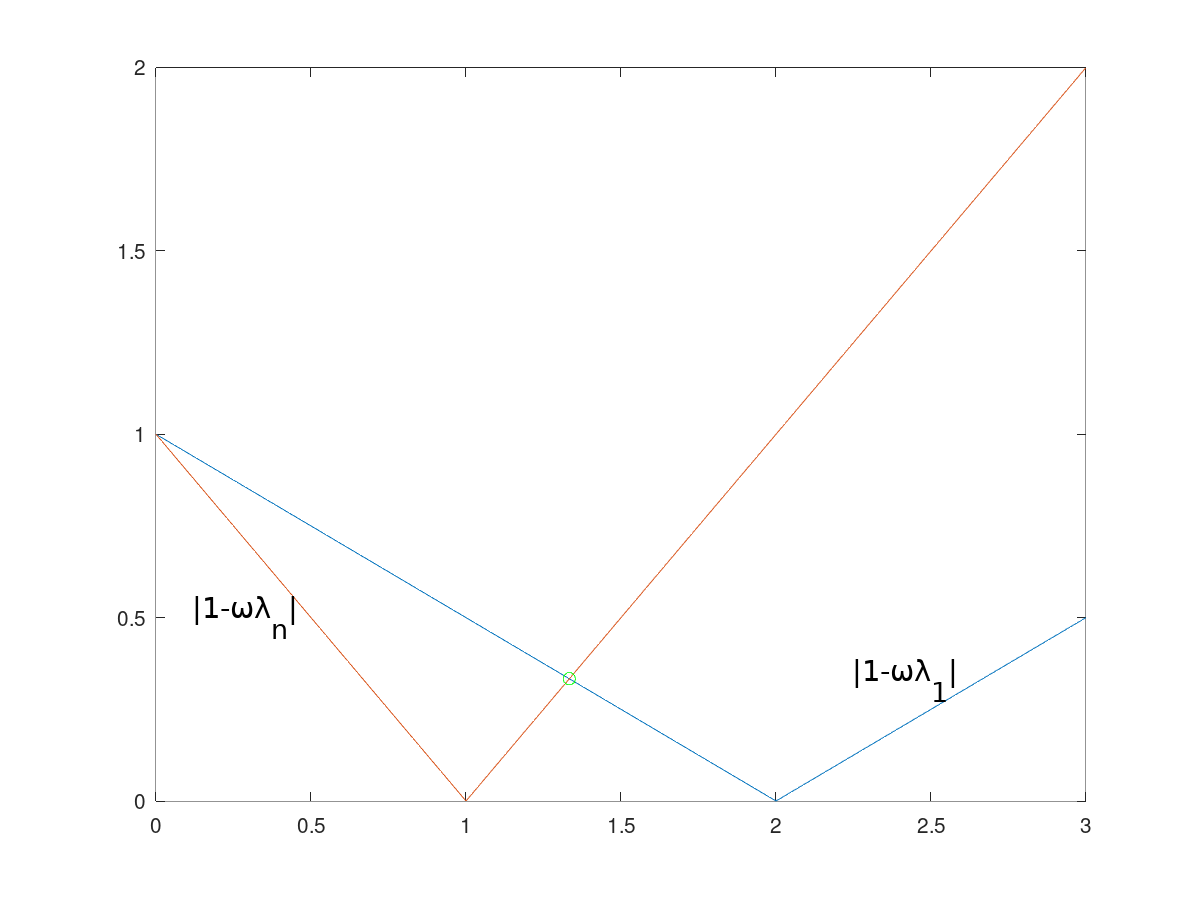
\includegraphics[width=0.4\linewidth]{modulos.png}
\end{figure}

se tiene
$$
\omega_{opt}=\frac{2}{\lambda_n+\lambda_1}
$$
de donde el respectivo
$$\rho(\Mb_I)=\frac{\lambda_n-\lambda_1}{\lambda_n+\lambda_1}=\frac{\kappa(\Ab)-1}{\kappa(\Ab)+1}.
$$
(Si $\kappa(\Ab)$ es muy grande la convergencia es muy lenta)

En el ejemplo del pricipio tenemos

$$
\lambda_1\sim 0.0009 \qquad \lambda_n \sim 1.93
$$

$$\kappa(\Ab)\sim 2144$$

$$\omega_{opt}\sim
1.04$$
$$\rho(\Mb_I)\sim 0.99907$$
si queremos un error del orden del orden de $10^{-5}$ precisamos iterar aproximadamente $15000$ veces, esto nos dio un tiempo de ejecución de $2.4 seg$ (recordemos que LU llevó $0.7 seg$ aun no es competitivo).




\begin{center}
 { \centering {Algunos Métodos Clásicos}}
\end{center}


Si tomamos $\Ab=\Lb+\Db+\Ub$ (triangular inferior+diagonal+triangular superior), podemos ensayar varias descomposiciones $\Ab=\Bb+\Cb$:
\begin{enumerate}
 \item $\Bb=\Db$ Jacobi
 \item $\Bb=\Lb+\Db$ Gauss-Seidel
\end{enumerate}

Las matrices de iteración son
\begin{enumerate}
 \item Jacobi $\Mb_J=-\Db^{-1}(\Lb+\Ub)$
 \item Gauss-Seidel $\Mb_{GS}=-(\Lb+\Db)^{-1}\Ub$
\end{enumerate}

Originalmente fueron concebidos de este modo:
de
$$
\Ab\xb=\bb,
$$
se tiene, para todo $1\le i\le n$
$$
\sum_{j=1}^na_{i,j}x_j=b_i,
$$

en Jacobi se escribe (asumiendo $a_{i,i}\neq0$)
$$
x_i=\left(-\sum_{j=1,j\neq i}^na_{i,j}x_j+b_i\right)/a_{i,i}\, \qquad \forall 1\le i\le n
$$
que da lugar al método
$$
x_i^{(k+1)}=\left(-\sum_{j=1,j\neq i}^na_{i,j}x_j^{(k)}+b_i\right)/a_{i,i}\, \qquad \forall 1\le i\le n
$$
para pasar del iterado $k$ al $k+1$.



Para Gauss-Seidel se escribe
$$
x_i^{(k+1)}=\left(-\sum_{j=i+1}^na_{i,j}x_j^{(k
)}-\sum_{j=1}^{i-1}a_{i,j}x_j^{(k+1)}+b_i\right)/a_{i,i}\, \qquad \forall 1\le i\le n
$$
para pasar del iterado $k$ al $k+1$, con la idea de  utilizar
$x_1^{(k+1)},\cdots x_{i-1}^{(k+1)}$ (considerados \emph{mejores} aproximaciones) en el cálculo de $x_i^{(k+1)}$.

Notar que:
\begin{itemize}
\item No es necesiario construir explícitamente $M_J$ no $M_{GS}$.
 \item Jacobi puede ``paralelizarse'' pero no así Gauss-Seidel.
\end{itemize}


\tccdefi
\begin{defi}
  \label{defi:deDD}
  Una matriz $\Ab\in \Knn$ se dice \emph{diagonal dominante} (\emph{estrictamente diagonal dominante}) y se denota DD (EDD) si y solo si para todo $i$,
 $1\le i\le n$
 $$
 \sum_{1\le j \le n, j\neq i}|a_{i,j}|\le (<) |a_{i,i}|.
 $$
  \end{defi}
 \etcc

\tcc
\begin{prop}
Sea $\Ab\in \Knn$ estrictamente diagonal dominante, entonces Jacobi y Gauss-Seidel convergen.
\end{prop}
\etcc
\begin{proof}
1. Jacobi: sea $\vb\in \Kn$ autovector de $\Mb_J$ de autovalor $\lambda$ q.v.q. $|\lambda|<1$.
$$
-D^{-1}(L+U)\vb=\lambda\vb,
$$
sea $1\le i\le n$ tal que
$0\neq |v_i|\ge |v_k|$ para todo $1\le k\le n$. Tenemos
$$
-\lambda v_ia_{i,i}=\sum_{i\neq j=1}^n a_{ij}v_j
$$, como $v_i\neq 0\neq a_{ii}$
$$
-\lambda=\sum_{i\neq j=1}^n \frac{a_{ij}v_j}{a_{ii}v_i}
$$
tomando modulo
$$
|\lambda|\le \sum_{i\neq j=1}^n |\frac{a_{ij}}{a_{ii}}|<1
$$
pues $\Ab$ es EDD.

2. Gauss-Seidel: como antes sea $\vb$ autovector de autovalor $\lambda$ de $\Mb_{GS}$, y $0\neq|v_i|\ge |v_k|$ con $1\le k\le n$:
$$
\Ub\vb=-\lambda(\Db+\Lb)\vb
$$
$$
\sum_{j=i+1}^na_{ij}\vb_j=-\lambda\left(
\sum_{j=1}^{i}a_{ij}\vb_j\right)
$$
dividiendo por $v_i$ y tomando módulos
$$
\sum_{j=i+1}^n|a_{ij}|
\ge \left|\sum_{j=i+1}^na_{ij}\frac{v_j}{v_i}\right|=|\lambda|\left|\left(
\sum_{j=1}^{i}a_{ij}\frac{v_j}{v_i}\right)\right|\ge |\lambda| \left(|a_{11}|-
\sum_{j=1}^{i-1}|a_{ij}|\right)
$$
de donde

$$
|\lambda|\le
\frac{\sum_{j=i+1}^n|a_{ij}|}{|a_{11}|-
\sum_{j=1}^{i-1}|a_{ij}|}
<1
$$
por ser EDD.
\end{proof}


El caso del ejemplo de la distribución de temperatura en el pistón no es EDD solamente DD.Sin embargo cumple con otras hipótesis que garantiza que Jacobi converge.


Para un error de $\sim 10^{-4}$ llevo 9000 iteraciones $\sim 1.9 seg$.

Tenemos un $\rho(M_J)\sim 0.998$.

(Igual es mucho mejor mirar el error relativo.)

Para GS por su parte pude probarse que converge para SDP (esta matriz es SDP).
En este caso $\rho(\Mb_{GS})\sim 0.996$, para un error de  $\sim 10^{-4}$ llevo 4500 iteraciones.

Que sea la mitad no es casual: se debe en este caso a que
$$
\rho(\Mb_{GS})=\rho(\Mb_{J})^2
$$
que ocurre típicamente en las matrices asociadas a estas ecuaciones difereciales

\tcc
\begin{prop}

 Si $\Ab\in\Knn$  DP, entonces Gauss-Seidel converge.
\end{prop}
\etcc
\begin{proof} Sea $\vb$ autovector de autovalor $\lambda$ de la matriz de iteraciones:
$$
-(\Db+\Lb)^{-1}\Ub\vb=\lambda\vb,
$$
$$
-\Ub\vb=\lambda(\Db+\Lb)\vb=\lambda \Ab \vb-\lambda \Ub
$$
$$
(\lambda-1)\Ub\vb=\lambda \Ab\vb
$$
$$
(\lambda-1)\vb^*\Ub\vb=\lambda \vb^*\Ab\vb
$$

$$
\frac{\lambda}{\lambda-1}=\frac{\vb^*\Ub\vb}{\vb^*\Ab\vb}
$$
como $\lambda\neq 1$ y $\Ab$ es Hermitiana (simétrica) $\Ub=\Lb^*$,
$$
2Re\left(\frac{\lambda}{\lambda-1}\right)=\frac{\vb^*(\Ub+\Lb)\vb}{\vb^*\Ab\vb}=\frac{\vb^*\Ub\vb}{\vb^*\Ab\vb}=1-\frac{\vb^*\Db\vb}{\vb^*\Ab\vb}<1.
$$
Llamando $\lambda=a+ib$ resulta
$$
2\frac{(a(a-1)+b^2)}{(a-1)^2+b^2}<1,
$$
y así
$|\lambda|^2=a^2+b^2<1.$
\end{proof}

Los métodos estudiados se originaron a partir de la identidad
$$
\xb=-\Bb^{-1}\Cb\xb+\Bb^{-1}\bb,
$$
que podemos reescribir
$$
\xb=\xb-\Bb^{-1}(\Ab\xb-\bb),
$$

y el método puede escribirse como la iteración
$$
\xb_{k+1}=\xb_k-\Bb^{-1}(\Ab\xb_k-\bb),
$$
que puede verse como una corrección que involucra al \emph{residuo} $\rb_k=\Ab\xb_k-\bb$

Por otro lado podemos tomar un  $0<\omega$ y escribir una nueva variante
$$
\xb_{j+1}=(1-\omega)\xb_j+
\omega(\xb_j-\Bb^{-1}(\Ab\xb_j-\bb)),
$$
dando mas o menos importancia a la iteración original.

Si $0<\omega<1$ el método se dice atenuado, si $\omega>1$ se dice amplificado.

Si aplicamos estas ideas a Gauss-Seidel obtenemos el método SOR. Para estudiarlo un poco reescribamos la iteración adecuadamente: de
$$
\xb^{k+1}=(1-\omega)\xb^k+
\omega(\xb^k-\Bb^{-1}(\Ab\xb^k-\bb)),
$$
tenemos
$$
\xb^{k+1}=(1-\omega)\xb^k+
\omega(-\Bb^{-1}\Cb\xb^k+\bb),
$$

en Gauss-Seidel tenemos $B=L+D$ y $C=U$, en particular podemos escribir en la coordenada $i-esima$:
$$
\xb^{k+1}_i=(1-\omega)\xb^k_i+
\frac{\omega}{a_{i,i}}(-\sum_{j=1}^{i-1}a_{i,j}\xb_j^{k+1}-\sum_{j=i+1}^{n}a_{i,j}\xb_j^k+\bb_i),
$$
o sea
$$
a_{i,i}\xb^{k+1}_i+\omega\sum_{j=1}^{i-1}a_{i,j}\xb_j^{k+1}=(1-\omega)a_{i,i}\xb^k_i-
\omega\sum_{j=i+1}^{n}a_{i,j}\xb_j^k -\omega\bb_i,
$$

En términos matriciales
$$
(\Db+\omega \Lb)\xb^{k+1}=\left((1-\omega)\Db-\omega\Ub\right)\xb^{k}-\omega \bb
$$
Es decir que el método tiene una matriz de iteraciones que puede escribirse
$$
\Mb_\omega=(\Db+\omega \Lb)^{-1}\left((1-\omega)\Db-\omega\Ub\right)
$$

En particular
$$
Det (\Mb_\omega)=(1-\omega)^n,
$$
y sabemos que
$\rho(\Mb_\omega)\ge |1-\omega|$
en particular, si el m\'etodo converge
$0<\omega<2$.

Ese resultado en general, pero para las matrices que son como las del ejemplo se puede probar que el método converge sí y solo sí
$0<\omega<2$
En cuanto al óptimo...
\begin{figure}[h]
\centering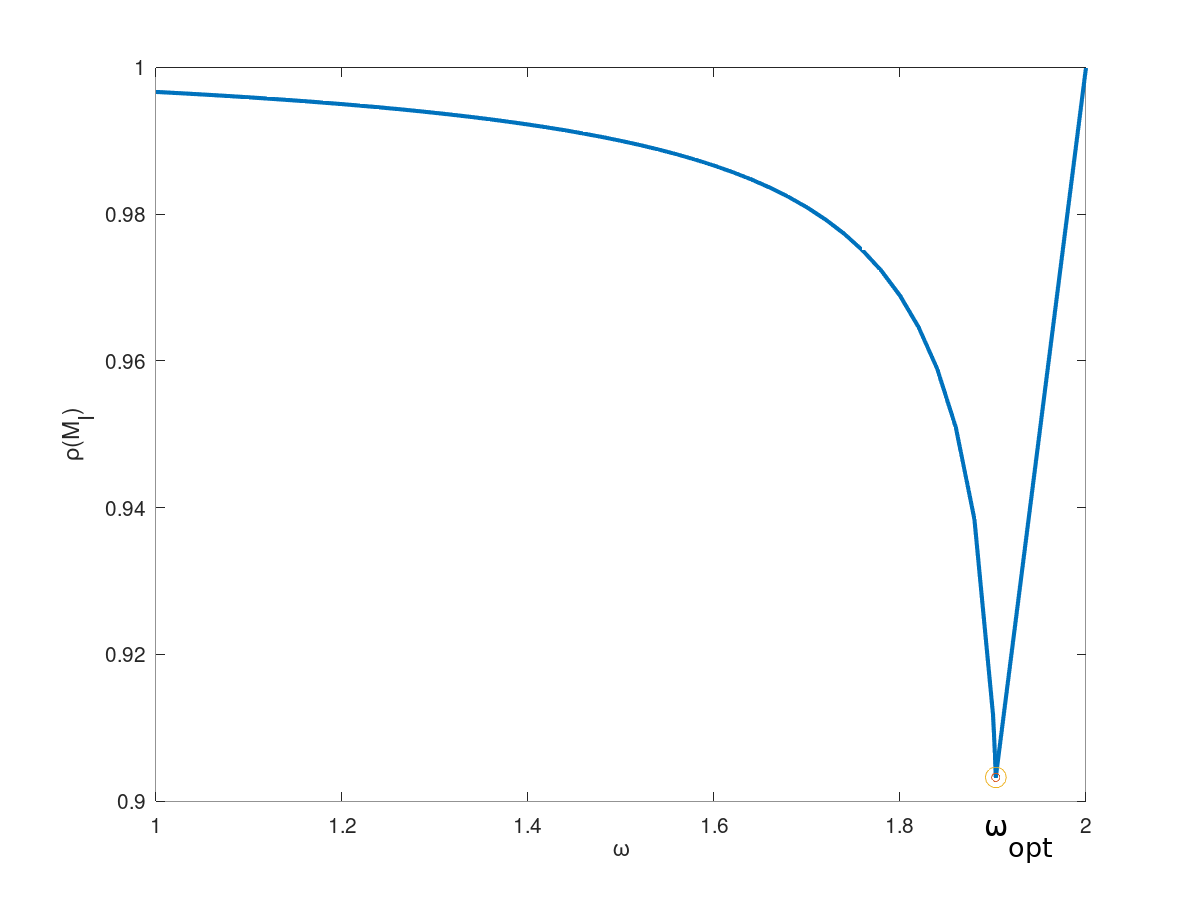
\includegraphics[width=0.6\linewidth]{omegaopt.png}
\end{figure}


En nuestro ejemplo:
tenemos $\omega_{opt}\sim 1.904$,
$$
\rho(\Mb_{\omega_{opt}})\sim 0.89
$$
tenemos un error de orden $10^{-4}$ en 150 iteraciones!.


Método de gradiente (o el descenso mas rápido)

Cuando trabajamos con matrices definidas positivas es posible reemplazar el problema:
$$
\mbox{(P1) Hallar $\xb\in \R^n$ tal que
}\,\Ab\xb=\bb
$$
por un problema de minimización  asociado a la función $J(\zb)=\frac{1}{2}\zb^*\Ab\zb-\zb^*\bb$:
$$
\mbox{(P2) Hallar $\xb\in \Rn$ tal que}\, J(\xb)=
\min_{\yb\in \R^n}J(\yb)
$$

Suponamos que $\xb$ resuelve (P1). Calculamos para $\zb\ne\cero$
$$
h(t)=J(\xb+t\zb)= \frac{1}{2}(\xb+t\zb)^*\Ab(\xb+t\zb)-(\xb+t\zb)^*\bb=
$$
$$
\frac{1}{2}t^2\zb^*\Ab\zb+t\left(\zb^*\Ab\xb-\zb^*\bb\right) +\frac{1}{2}\xb^*\Ab\xb-\xb^*\bb
$$
cuadr\'atica con mínimo en
$$
t=\frac{\zb^*\Ab\xb-\zb^*\bb}{\zb^*\Ab\zb}=0
$$
pues $\Ab\xb=\bb$.

Entonces
$$
J(\xb)=h(0)\le h(t)=J(\xb+t\zb)
$$
para todo $t$ entonces
$$
J(\xb)=\min_{\yb\in\Rn}J(\yb).
$$

Recíprocamente: si
$$
J(\xb)=\min_{\yb\in\Rn}J(\yb),
$$
repetimos la cuenta anterior y vemos que el mínimo de $h(t)$ está en $t=0$ lo que dice que
$$0=\frac{\zb^*\Ab\xb-\zb^*\bb}{\zb^*\Ab\zb}
$$
es decir
$$
\zb^*(\Ab\xb-\bb)=0,
$$
para todo $\zb\neq \cero$.


Tomando $\zb=\eb_1,\eb_2,\cdots \eb_n$ resulta
$$
\Ab\xb-\bb=\cero,
$$
es decir
$$
\Ab\xb=\bb.
 $$


\section{M\'etodos Iterativos no Estacionarios}
Los métodos no estacionarios difieren en lo estacionarios en que típicamente involucran información que cambia en cada interación
\section{Método del Gradiente, o del descenso mas rápido}

\section{Gradiente Conjugado}
Se trata de un método muy efectivo y ampliamente utilizado para matrices \emph{simétricas definida positivas}. El método funciona generando una sucesión de iterados -que aproximan a la solución- y de residuos correspondientes a los iterados junto con las direcciones de búsqueda para actualizar los nuevos iterados y junto con sus residuos actualizados.

En cada iteración solo unos pocos vectores necesitan guardarse en memoria. Solo dos productos internos son necesarios para calcular los escalares que hacen que la sucesión resultante satisfaga ciertas propiedades de ortogonalidad. y los escalares

\tcc
Para matrices simétricas, definidas positivas, el Método del Gradiente Conjuado garantiza que en cada iteración se minimiza la distancia a la solución exacta en cierta norma.
\etcc

En cada paso los iterados $\xb_i$ se actualizan a través de un múltiplo $\alpha_i$ de una cierta dirección de  búsqueda $\pb_i$
$$
\xb_i=\xb_{i-1}+\alpha_i\pb_i,
$$
los residuos $\rb_i=\bb-\Ab\xb_i$ pueden actualizarse a través de la ecuación previa
$$
\rb_i=\rb_{i-1}-\alpha_i\qb_i,
$$
con $\qb_i=\Ab\pb_i$.
La elección $\alpha_i=\frac{\rb_{i-1}^T\rb_{i-1}}{\pb_{i-1}^T\Ab\pb_{i-1}}$,
minimiza la expresión $\rb_{i-1}^T\Ab^{-1}\rb_{i-1}$ entre todos los
$\alpha\in \R$.

Las direcciones de busqueda se actualizan con los residuos
$$
\pb_i=\rb_i+\beta_{i-1}\pb_{i-1},?
$$
donde la elección
$$
\beta_{i}=\frac{\rb_{i}^T\rb_{i}}{\rb_{i-1}^T\rb_{i-1}},
$$
garantiza que $\pb_i$ y $\Ab\pb_i$ (o equivalentemente $\rb_i$ y $\rb_{i-1}$)- son ortogonales.

Mas aún, esta elección de $\beta_i$, tanto $\pb_i$ como $\rb_i$ son ortogonales \emph{a todos los anteriores} $\pb_j$ y $\rb_j$ ($j<i$) respectivamente.

(esto salio de pagina 13 de Templates for te solution of linear systems....)


\section{Aplicaciones de SVD}
\begin{itemize}
 \item compresión de imágenes
\item semántica latente
\item componentes principales
\end{itemize}
